\documentclass[10pt]{article}

\usepackage{graphicx}
\usepackage{epstopdf}
\usepackage{float}
\usepackage[T1]{fontenc}
\usepackage[titletoc]{appendix}
\usepackage[margin=0.7in]{geometry}
\usepackage{blindtext}
\usepackage[english]{babel}
\usepackage{multirow}
\usepackage{courier}
\usepackage{fancyhdr}
\usepackage{makecell}
\usepackage{caption}
\usepackage{rotating}
\usepackage{pdflscape}
\pagestyle{fancy}
\lhead{Tim Yao - ty252}

\renewcommand{\thesubsection}{\thesection.\alph{subsection}}

\usepackage{listings}
\usepackage{color}

\definecolor{dkgreen}{rgb}{0,0.6,0}
\definecolor{gray}{rgb}{0.5,0.5,0.5}
\definecolor{mauve}{rgb}{0.58,0,0.82}

\lstset{frame=tb,
  language=Verilog,
  aboveskip=3mm,
  belowskip=3mm,
  showstringspaces=false,
  columns=flexible,
  keepspaces=true,
  numbers=left,
  basicstyle={\small\ttfamily},
  keywordstyle=\color{blue},
  commentstyle=\color{dkgreen},
  stringstyle=\color{mauve},
  breaklines=false,
  breakatwhitespace=true,
  tabsize=2
}

% For monospace stuff

\title{ECE 4750 PSET 3}
\author{Tim Yao (ty252)}
\date{Nov 6, 2015}

\begin{document}
\maketitle
\newcommand*{\tableindent}{\hspace*{0.3cm}}%

\section{Tree Network Topologies} 

\begin{figure}[H]
\centering
\begin{tabular}{@{\extracolsep{3pt}}llcccc@{}}
\Xhline{2\arrayrulewidth}
& & & \textit{b} & & $\Theta_{term}$ \\
\textbf{Part} & \textbf{Topology} & $B_c$ & {(bits/cycle)} & $\gamma_{max}$ & {(bits/cycle)} \\
\hline
\textbf{Part 1.A} & \textbf{Baseline Tree Topology} & 2 & 32 & 2 & 16 \\
\hline
\textbf{Part 1.B} & \textbf{Fat-Tree Topology} & 8 & 32 & 1 & 32  \\
\Xhline{2\arrayrulewidth}
\end{tabular}
\caption{Ideal Terminal Throughput for Tree Topologies}
\end{figure}

\begin{figure}[H]
\centering
\begin{tabular}{@{\extracolsep{3pt}}llccccccc@{}}
\Xhline{2\arrayrulewidth}
& & & & \textit{$t_r$} & & \textit{$t_c$} & \textit{$L/b$} & \textit{$t_0$}\\
\textbf{Part} & \textbf{Topology} & \textit{$H_D$} & \textit{$H_r$} & (cycles) & \textit{$H_c$} & (cycle) & (cycle) & (cycle) \\
\hline
\textbf{Part 1.A} & \textbf{Baseline Tree Topology} & 4 & 3 & 2 & 2 & 1 & 3 & 11\\
\hline
\textbf{Part 1.B} & \textbf{Fat-Tree Topology} & 4 & 3 & 3.83 & 2 & 1 & 3 & 16.5\\
\Xhline{2\arrayrulewidth}
\end{tabular}
\caption{Zero-Load Latency for Tree Topologies}
\end{figure}

\subsection{Performance of Baseline Tree Topology}
To calculate the minimum bisection channel count, I first found the minimum bisection cut. This happens to be the cut on the channels that connect the two level-2 routers. This cut cuts 2 channels, so the $B_c$ is 2. \\
To calculate the max channel, there are 3 possibilities. It can be the channels connecting between the nodes and the level-1 routers, level-1 and level-2 routers, and between the two level-2 routers. Because we are dealing with uniform random routing, all channels of one level has the same load.\\
The channel load for channels between nodes and level-1 routers are 1. In uniform random routing, the amount traffic sent from and to a node is always equal to 1. \\
The channel load for channels between level-1 and level-2 routers are 1.5. To calculate this, I first look at the amount of traffic that is sent from one node to all other nodes that require crossing the this channel. For example, all traffic that go from node 0 to 2,3,4,5,6,7 need to cross this channel. Each unit of traffic is 1/8, so for each node that resides under (in the sense of a tree) that channel is 6/8. Because there are 2 nodes (ie. node 0 and 1) under that channel, the max channel load is 2*6/8 = 12/8 = 3/2.\\
The channel load for channels between level-2 routers are 2. We use the same idea from the previous calculation to calculate this max load. Each node on the left side needs to send to 4 nodes on the right side, therefore, each node contributes 4*1/8 = 1/2 unit of traffic. There are 4 nodes, so the max load is 4*1/2 = 2.
From this, we see that the max channel load is between the two level 2 routers. And using the ideal terminal throughput equation, $\Theta_{term}$=$B_c$/$\gamma_{max}$, I calculated that $\Theta_{term}$=32/2=16.\\
\\
The network diameter is 4 router hops. One example is the path going from node 0 to node 7. This minimum path takes 4 router hops.\\
The average number of router hops is calculated using the following method. The average number of router hops for going from 0 to itself and all other nodes is the same from 1 to itself and all other nodes, from 2 to itself and all other nodes, and etc. Therefore, we can calculate the overall average number of router hops by simply analyzing the traffic going from 1 node to itself and all other nodes. If we pick 0, then the analysis is as following:\\
0->0: 1\\
0->1: 1\\
0->2: 3\\
0->3: 3\\
0->4: 4\\
0->5: 4\\ 
0->6: 4\\ 
0->7: 4\\ 
The average is then: (1+1+3+3+4+4+4+4)/8=24/8=3 hops.\\
Because all of the routers are radix-2, the average per-hop router latency is 2.\\
The method to calculate the average channel hop count is the same as calculating the average router hop count. \\
0->0: 0\\
0->1: 0\\
0->2: 2\\
0->3: 2\\
0->4: 3\\
0->5: 3\\ 
0->6: 3\\ 
0->7: 3\\
The average is then: (2+2+3+3+3+3)/8=16/8=2 hops.\\
The average per-hop channel latency is 1 cycle as stated in the assumption.\\
Because the message is 96 bits and the channel width is 32 bits, the serialization latency is 96/32=3 cycles.\\
Now, we can calculate the zero-load latency.\\
$t_0$=$H_r$$t_r$+$H_c$$t_c$+L/b\\
$t_0$=3*2+2*1+3=11 cycles
\subsection{Performance of Fat-Tree Topology}
We use the same approach as in the previous section to calculate the max channel load and ideal terminal throughput for the baseline tree topology. Again, the channels connecting nodes to level-1 routers have a load of 1. The total load on all channels between level-1 and level-2 routers are the same (because this is a uniforma random traffic pattern), but now there are twice the number of channels. Therefore, the channel load is 6/8=3/4. The total load on all channels between the two level-2 routers are also the same, but because there are now 4 times the number of channels, the channel load is 1/2. Therefore, the max channel load is on the channels between nodes and level-1 routers. The max channel load is 1 and the ideal terminal throughput is 32/1=32.\\
\\
Because the layout topology and channel width of the fat-tree is the same as the baseline, the network diameter, average router hop count, average channel hop count, average per-hop channel latency, and serialization latency are the same.\\
The only difference here is the average per-hop router latency due to different radix routers. To calculate this, we take a similar approach to calculating the average hop counts. We use a weighted average for each node-pair due to the different latencies of different routers.\\
0->0: 3\\
0->1: 3\\
0->2: 3+5+3 = 11\\
0->3: 3+5+3 = 11\\
0->4: 3+5+5+3 = 16\\
0->5: 3+5+5+3 = 16\\ 
0->6: 3+5+5+3 = 16\\ 
0->7: 3+5+5+3 = 16\\
The average is: (3+3+11+11+16+16+16+16)/24=92/24=23/6=3.833\\
From this, we can calculate the zero-load latency.\\
$t_0$=3*23/6+2*1+3=16.5 cycles
\subsection{Integrating Processors, Memories, and Networks}

\cleardoublepage
\section{Channel and Router Microarchitecture}

\subsection{Throughput with One Element of Buffering per Channel Queue}

\begin{figure}[H]
\centering
{\setlength{\tabcolsep}{2pt}
\begin{tabular}{|l|c|c|c|c|c|c|c|c|c!{\vrule width 1.5pt}c|c!{\vrule width 1.5pt}c|c!{\vrule width 1.5pt}c|c!{\vrule width 1.5pt}c|c!{\vrule width 1.5pt}c|c!{\vrule width 1.5pt}c|}
\hline
Cycle: & 1  & 2  & 3  & 4  & 5  & 6  & 7  & 8  & 9  & 10 & 11 & 12 & 13 & 14 & 15 & 16 & 17 & 18 & 19 & 20 \\ \hline
pkt0   & I  & R0 & L0 & L1 & R1 & O  &    &    &    &    &    &    &    &    &    &    &    &    &    &    \\ \hline
pkt1   &    & I  & R0 & R0 & L0 & L1 & R1 & O  &    &    &    &    &    &    &    &    &    &    &    &    \\ \hline
pkt2   &    &    & I  & q  & R0 & R0 & L0 & L1 & R1 & O  &    &    &    &    &    &    &    &    &    &    \\ \hline
pkt3   &    &    &    & I  & I  & q  & R0 & R0 & L0 & L1 & R1 & O  &    &    &    &    &    &    &    &    \\ \hline
pkt4   &    &    &    &    &    & I  & I  & q  & R0 & R0 & L0 & L1 & R1 & O  &    &    &    &    &    &    \\ \hline
pkt5   &    &    &    &    &    &    &    & I  & I  & q  & R0 & R0 & L0 & L1 & R1 & O  &    &    &    &    \\ \hline
pkt6   &    &    &    &    &    &    &    &    &    & I  & I  & q  & R0 & R0 & L0 & L1 & R1 & O  &    &    \\ \hline
pkt7   &    &    &    &    &    &    &    &    &    &    &    & I  & I  & q  & R0 & R0 & L0 & L1 & R1 & O  \\ \hline
\end{tabular}
}
\caption{Pipeline Diagram for Elastic Buffering with One-Element Channel Buffers}
\end{figure}
As show by the bolded vertical lines, in steady state, it takes 2 cycles to move a packet. This gives a peak terminal throughput of 1/2=0.5 packets per cycle.

\subsection{Throughput with Two Elements of Buffering per Channel Queue}

\begin{figure}[H]
\centering
{\setlength{\tabcolsep}{2pt}
\begin{tabular}{|l|c|c|c|c|c|c|c|c|c!{\vrule width 1.5pt}c!{\vrule width 1.5pt}c!{\vrule width 1.5pt}c!{\vrule width 1.5pt}c|}
\hline
Cycle: & 1  & 2  & 3  & 4  & 5  & 6  & 7  & 8  & 9  & 10 & 11 & 12 & 13 \\ \hline
pkt0   & I  & R0 & L0 & L1 & R1 & O  &    &    &    &    &    &    &    \\ \hline
pkt1   &    & I  & R0 & L0 & L1 & R1 & O  &    &    &    &    &    &    \\ \hline
pkt2   &    &    & I  & R0 & L0 & L1 & R1 & O  &    &    &    &    &    \\ \hline
pkt3   &    &    &    & I  & R0 & L0 & L1 & R1 & O  &    &    &    &    \\ \hline
pkt4   &    &    &    &    & I  & R0 & L0 & L1 & R1 & O  &    &    &    \\ \hline
pkt5   &    &    &    &    &    & I  & R0 & L0 & L1 & R1 & O  &    &    \\ \hline
pkt6   &    &    &    &    &    &    & I  & R0 & L0 & L1 & R1 & O  &    \\ \hline
pkt7   &    &    &    &    &    &    &    & I  & R0 & L0 & L1 & R1 & O  \\ \hline
\end{tabular}
}
\caption{Pipeline Diagram for Elastic Buffering with Two-Element Channel Buffers}
\end{figure}
As show by the bolded vertical lines, in steady state, it takes 1 cycle to move a packet. This gives a peak terminal throughput of 1 packet per cycle.

\subsection{Pipeline Diagram for Round-Robin Arbitration}

\begin{figure}[H]
\centering
{\setlength{\tabcolsep}{2pt}
\begin{tabular}{|l|c|c|c|c|c|c|c|c|c|c|c|c|c|}
\hline
Cycle: & 1  & 2  & 3  & 4  & 5  & 6  & 7  & 8  & 9  & 10 & 11 & 12 & 13 \\ \hline
pkt0-2 & I  & R0 & L0 & L1 & R1 & O  &    &    &    &    &    &    &    \\ \hline
pkt0-3 & I  & R0 & R0 & L0 & L1 & R1 & O  &    &    &    &    &    &    \\ \hline
pkt1-2 &    & I  & R0 & R0 & L0 & L1 & R1 & O  &    &    &    &    &    \\ \hline
pkt1-3 &    & I  & q  & R0 & R0 & L0 & L1 & R1 & O  &    &    &    &    \\ \hline
pkt2-2 &    &    & I  & q  & R0 & R0 & L0 & L1 & R1 & O  &    &    &    \\ \hline
pkt2-3 &    &    & I  & q  & q  & R0 & R0 & L0 & L1 & R1 & O  &    &    \\ \hline
pkt3-2 &    &    &    & I  & q  & q  & R0 & R0 & L0 & L1 & R1 & O  &    \\ \hline
pkt3-3 &    &    &    & I  & q  & q  & q  & R0 & R0 & L0 & L1 & R1 & O  \\ \hline
\end{tabular}
}
\caption{Pipeline Diagram for Round-Robin Arbitration}
\end{figure}
There is no steady state. As shown by the pipeline diagram, the number of elements in the $R_{0,1}$ queue continues to increase. This is due to the the $C_{0,3}$ channel not able to sustain the required throughput (2 phits per cycle). This means that packets will need to be stalled in R0 during arbitration and therefore cause future packets to be continuously queued up. 

\subsection{Global Fairness for Round-Robin Arbitration}


\cleardoublepage
\section{In-Order Superscalar Processors}

\subsection{Pipeline Diagram for Single-Issue PARCv1 Processor}

\begin{figure}[H]
\centering
{\setlength{\tabcolsep}{2pt}
\begin{tabular}{|l|c|c|c|c!{\vrule width 1.5pt}c|c|c|c|c|c|c|c|c|c|c|c!{\vrule width 1.5pt}c|c|}
\hline
Cycle:            & 1 & 2 & 3 & 4 & 5 & 6 & 7 & 8 & 9 & 10 & 11 & 12 & 13 & 14 & 15 & 16 & 17 & 18 \\ \hline
lw r1 , 0(r2)     & F & D & X & M & W &   &   &   &   &    &    &    &    &    &    &    &    &    \\ \hline
lw r3 , 0(r4)     &   & F & D & X & M & W &   &   &   &    &    &    &    &    &    &    &    &    \\ \hline
mul r1, r1, r6    &   &   & F & D & X & M & W &   &   &    &    &    &    &    &    &    &    &    \\ \hline
mul r3, r3, r7    &   &   &   & F & D & X & M & W &   &    &    &    &    &    &    &    &    &    \\ \hline
addu r8, r1, r3   &   &   &   &   & F & D & X & M & W &    &    &    &    &    &    &    &    &    \\ \hline
addu r9, r9, r8   &   &   &   &   &   & F & D & X & M & W  &    &    &    &    &    &    &    &    \\ \hline
addiu r2, r2, 4   &   &   &   &   &   &   & F & D & X & M  & W  &    &    &    &    &    &    &    \\ \hline
addiu r4, r4, 4   &   &   &   &   &   &   &   & F & D & X  & M  & W  &    &    &    &    &    &    \\ \hline
addiu r10, r10, -1&   &   &   &   &   &   &   &   & F & D  & X  & M  & W  &    &    &    &    &    \\ \hline
bne r10, r0, loop &   &   &   &   &   &   &   &   &   & F  & D  & X  & M  & W  &    &    &    &    \\ \hline
opA               &   &   &   &   &   &   &   &   &   &    & F  & D  & -  & -  & -  &    &    &    \\ \hline
opB               &   &   &   &   &   &   &   &   &   &    &    & F  & -  & -  & -  & -  &    &    \\ \hline
lw r1 , 0(r2)     &   &   &   &   &   &   &   &   &   &    &    &    & F  & D  & X  & M  & W  &    \\ \hline
lw r3 , 0(r4)     &   &   &   &   &   &   &   &   &   &    &    &    &    & F  & D  & X  & M  & W  \\ \hline
\end{tabular}
}
\caption{Pipeline Diagram for Single-Issue PARCv1 Processor}
\end{figure}
As shown by the bold vertical lines, each loop takes 12 cycles to execute. The CPI is therefore 12/10 = 1.2. The IPC is 1/CPI = 0.833.\\
CPI = 1.2 cycles/instruction\\
IPC = 0.83 instructions/cycle\\

\subsection{Pipeline Diagram for Dual-Issue PARCv1 Processor}

\begin{figure}[H]
\centering
{\setlength{\tabcolsep}{2pt}
\begin{tabular}{|l|c|c|c|c!{\vrule width 1.5pt}c|c|c|c|c|c|c|c|c|c|c!{\vrule width 1.5pt}c|c|}
\hline
Cycle:            & 1  & 2  & 3  & 4  & 5  & 6  & 7  & 8  & 9  & 10 & 11 & 12 & 13 & 14 & 15 & 16 & 17 \\ \hline
lw r1 , 0(r2)     & F  & D  & B0 & B1 & W  &    &    &    &    &    &    &    &    &    &    &    &    \\ \hline
lw r3 , 0(r4)     & F  & D  & D  & B0 & B1 & W  &    &    &    &    &    &    &    &    &    &    &    \\ \hline
mul r1, r1, r6    &    & F  & F  & D  & A0 & A1 & W  &    &    &    &    &    &    &    &    &    &    \\ \hline
mul r3, r3, r7    &    & F  & F  & D  & D  & A0 & A1 & W  &    &    &    &    &    &    &    &    &    \\ \hline
addu r8, r1, r3   &    &    &    & F  & F  & D  & A0 & A1 & W  &    &    &    &    &    &    &    &    \\ \hline
addu r9, r9, r8   &    &    &    & F  & F  & D  & D  & B0 & B1 & W  &    &    &    &    &    &    &    \\ \hline
addiu r2, r2, 4   &    &    &    &    &    & F  & F  & D  & A0 & A1 & W  &    &    &    &    &    &    \\ \hline
addiu r4, r4, 4   &    &    &    &    &    & F  & F  & D  & B0 & B1 & W  &    &    &    &    &    &    \\ \hline
addiu r10, r10, -1&    &    &    &    &    &    &    & F  & D  & B0 & B1 & W  &    &    &    &    &    \\ \hline
bne r10, r0, loop &    &    &    &    &    &    &    & F  & D  & D  & A0 & A1 & W  &    &    &    &    \\ \hline
opA               &    &    &    &    &    &    &    &    & F  & F  & D  & -  & -  & -  &    &    &    \\ \hline
opB               &    &    &    &    &    &    &    &    & F  & F  & D  & -  & -  & -  &    &    &    \\ \hline
opC               &    &    &    &    &    &    &    &    &    &    & F  & -  & -  & -  & -  &    &    \\ \hline
opD               &    &    &    &    &    &    &    &    &    &    & F  & -  & -  & -  & -  &    &    \\ \hline
lw r1 , 0(r2)     &    &    &    &    &    &    &    &    &    &    &    & F  & D  & B0 & B1 & W  &    \\ \hline
lw r3 , 0(r4)     &    &    &    &    &    &    &    &    &    &    &    & F  & D  & D  & B0 & B1 & W  \\ \hline
\end{tabular}
}
\caption{Pipeline Diagram for Dual-Issue PARCv1 Processor}
\end{figure}
As shown by the bold vertical lines, each loop takes 11 cycles to execute. The CPI is therefore 11/10 = 1.1. The IPC is 1/CPI = 0.910.\\
CPI = 1.1 cycles/instruction\\
IPC = 0.91 instructions/cycle\\

\subsection{Optimized Pipeline Diagram for Dual-Issue PARCv1 Processor}

\begin{lstlisting}
lw r1 , 0(r2)     
addiu r2, r2, 4   
lw r3 , 0(r4)     
addiu r4, r4, 4   
mul r1, r1, r6    
addiu r10, r10, -1
mul r3, r3, r7    
addu r8, r1, r3   
addu r9, r9, r8   
bne r10, r0, loop                
\end{lstlisting}

\begin{figure}[H]
\centering
{\setlength{\tabcolsep}{2pt}
\begin{tabular}{|l|c|c|c|c!{\vrule width 1.5pt}c|c|c|c|c|c|c|c!{\vrule width 1.5pt}c|}
\hline
Cycle:            & 1  & 2  & 3  & 4  & 5  & 6  & 7  & 8  & 9  & 10 & 11 & 12 & 13 \\ \hline
lw r1 , 0(r2)     & F  & D  & B0 & B1 & W  &    &    &    &    &    &    &    &    \\ \hline
addiu r2, r2, 4   & F  & D  & A0 & A1 & W  &    &    &    &    &    &    &    &    \\ \hline
lw r3 , 0(r4)     &    & F  & D  & B0 & B1 & W  &    &    &    &    &    &    &    \\ \hline
addiu r4, r4, 4   &    & F  & D  & A0 & A1 & W  &    &    &    &    &    &    &    \\ \hline
mul r1, r1, r6    &    &    & F  & D  & A0 & A1 & W  &    &    &    &    &    &    \\ \hline
addiu r10, r10, -1&    &    & F  & D  & B0 & B1 & W  &    &    &    &    &    &    \\ \hline
mul r3, r3, r7    &    &    &    & F  & D  & A0 & A1 & W  &    &    &    &    &    \\ \hline
addu r8, r1, r3   &    &    &    & F  & D  & D  & B0 & B1 & W  &    &    &    &    \\ \hline
addu r9, r9, r8   &    &    &    &    & F  & F  & D  & B0 & B1 & W  &    &    &    \\ \hline
bne r10, r0, loop &    &    &    &    & F  & F  & D  & A0 & A1 & W  &    &    &    \\ \hline
opA               &    &    &    &    &    &    & F  & D  & -  & -  & -  &    &    \\ \hline
opB               &    &    &    &    &    &    & F  & D  & -  & -  & -  &    &    \\ \hline
opC               &    &    &    &    &    &    &    & F  & -  & -  & -  & -  &    \\ \hline
opD               &    &    &    &    &    &    &    & F  & -  & -  & -  & -  &    \\ \hline
lw r1 , 0(r2)     &    &    &    &    &    &    &    &    & F  & D  & B0 & B1 & W  \\ \hline
addiu r2, r2, 4   &    &    &    &    &    &    &    &    & F  & D  & A0 & A1 & W  \\ \hline
\end{tabular}
}
\caption{Optimized Pipeline Diagram for Dual-Issue PARCv1 Processor}
\end{figure}

As shown by the bold vertical lines, each loop takes 8 cycles to execute. The CPI is therefore 8/10 = 0.8. The IPC is 1/CPI = 1.25.\\
CPI = 0.8 cycles/instruction\\
IPC = 1.25 instructions/cycle

\subsection{Optimized Pipeline Diagram for Quad-Issue PARCv1 Processor}

\begin{lstlisting}
lw r1 , 0(r2)     
addiu r2, r2, 4   
lw r3 , 0(r4)     
addiu r4, r4, 4   
mul r1, r1, r6    
addiu r10, r10, -1
mul r3, r3, r7    
addu r8, r1, r3   
addu r9, r9, r8   
bne r10, r0, loop                
\end{lstlisting}

\begin{figure}[H]
\centering
{\setlength{\tabcolsep}{2pt}
\begin{tabular}{|l|c|c|c|c!{\vrule width 1.5pt}c|c|c|c|c|c|c!{\vrule width 1.5pt}c|}
\hline
Cycle:            & 1  & 2  & 3  & 4  & 5  & 6  & 7  & 8  & 9  & 10 & 11 & 12 \\ \hline
lw r1 , 0(r2)     & F  & D  & B0 & B1 & W  &    &    &    &    &    &    &    \\ \hline
addiu r2, r2, 4   & F  & D  & A0 & A1 & W  &    &    &    &    &    &    &    \\ \hline
lw r3 , 0(r4)     & F  & D  & H0 & H1 & W  &    &    &    &    &    &    &    \\ \hline
addiu r4, r4, 4   & F  & D  & G0 & G1 & W  &    &    &    &    &    &    &    \\ \hline
mul r1, r1, r6    &    &    & F  & D  & A0 & A1 & W  &    &    &    &    &    \\ \hline
addiu r10, r10, -1&    &    & F  & D  & B0 & B1 & W  &    &    &    &    &    \\ \hline
mul r3, r3, r7    &    &    & F  & D  & G0 & G1 & W  &    &    &    &    &    \\ \hline
addu r8, r1, r3   &    &    & F  & D  & D  & H0 & H1 & W  &    &    &    &    \\ \hline
addu r9, r9, r8   &    &    &    & F  & F  & D  & B0 & B1 & W  &    &    &    \\ \hline
bne r10, r0, loop &    &    &    & F  & F  & D  & A0 & A1 & W  &    &    &    \\ \hline
opA               &    &    &    & F  & F  & D  & G0 & -  & -  &    &    &    \\ \hline
opB               &    &    &    & F  & F  & D  & H0 & -  & -  &    &    &    \\ \hline
opC               &    &    &    &    &    & F  & D  & -  & -  & -  &    &    \\ \hline
opD               &    &    &    &    &    & F  & D  & -  & -  & -  &    &    \\ \hline
opE               &    &    &    &    &    & F  & D  & -  & -  & -  &    &    \\ \hline
opF               &    &    &    &    &    & F  & D  & -  & -  & -  &    &    \\ \hline
opG               &    &    &    &    &    &    & F  & -  & -  & -  & -  &    \\ \hline
opH               &    &    &    &    &    &    & F  & -  & -  & -  & -  &    \\ \hline
opI               &    &    &    &    &    &    & F  & -  & -  & -  & -  &    \\ \hline
opJ               &    &    &    &    &    &    & F  & -  & -  & -  & -  &    \\ \hline
lw r1 , 0(r2)     &    &    &    &    &    &    &    & F  & D  & B0 & B1 & W  \\ \hline
addiu r2, r2, 4   &    &    &    &    &    &    &    & F  & D  & A0 & A1 & W  \\ \hline
lw r3 , 0(r4)     &    &    &    &    &    &    &    & F  & D  & H0 & H1 & W  \\ \hline
addiu r4, r4, 4   &    &    &    &    &    &    &    & F  & D  & G0 & G1 & W  \\ \hline
\end{tabular}
}
\caption{Optimized Pipeline Diagram for Dual-Issue PARCv1 Processor}
\end{figure}

As shown by the bold vertical lines, each loop takes 7 cycles to execute. The CPI is therefore 7/10 = 0.7. The IPC is 1/CPI = 1.43.\\
CPI = 0.7 cycles/instruction\\
IPC = 1.43 instructions/cycle

\subsection{Instruction Level Parallelism}

\begin{figure}[H]
\begin{center}
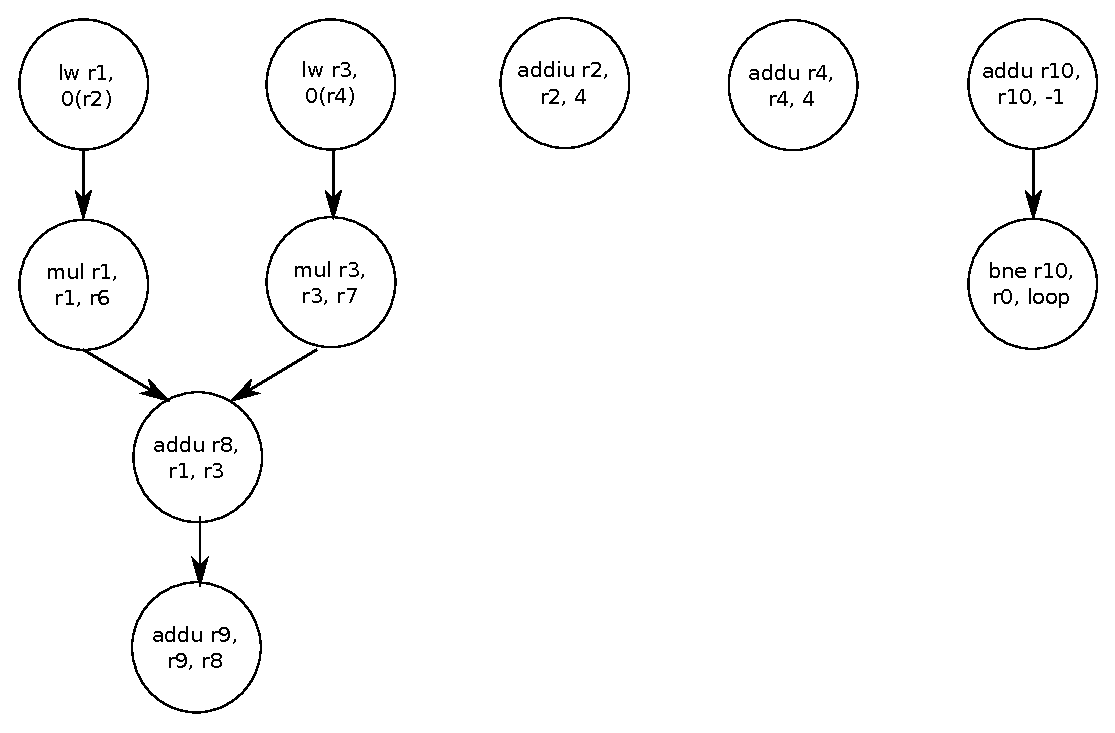
\includegraphics[scale=0.5]{singleiteri.eps}
\label{default}
\end{center}
\caption{Instruction Dependency Graph for Single Iteration}
\end{figure}
The longest path contains 4 nodes.
The ideal ILP for a single iteration is 10/4 = 2.5.

\begin{figure}[H]
\begin{center}
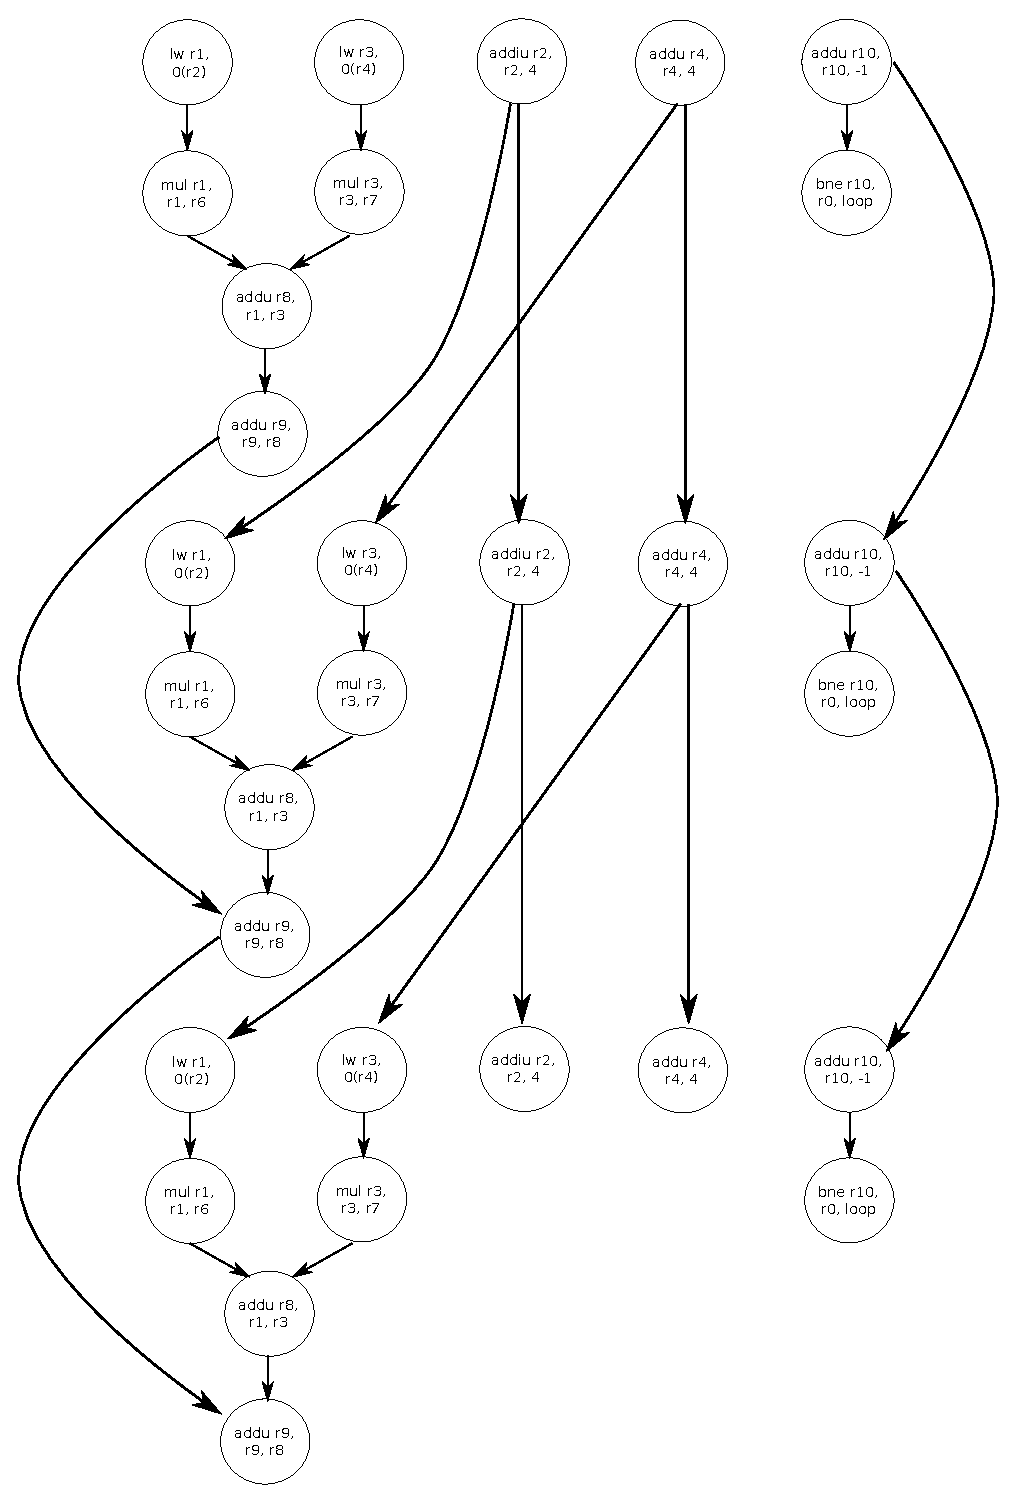
\includegraphics[scale=0.7]{threeiteri.eps}
\label{default}
\end{center}
\caption{Instruction Dependency Graph for Three Iterations}
\end{figure}
The longest path contains 6 nodes. 
The ideal ILP for three iterations is 30/6 = 5.\\

The ideal ILP for N iterations of the loop is simply 10N/(3+N).\\

The IPC of the quad-issue processor is less than the ideal ILP due to several different reasons. The first is that the quad issue processor can only execute at most 4 instructions simultaneously. This thereby limits the IPC to a max of 4. 

\end{document}